\frame{
  \frametitle{Molecular biology time series}
    \begin{flushright}
    \textbf{Antti Honkela}
    \end{flushright}

  \begin{itemize}
  \item Biological systems are dynamic, observing their time evolution
    very helpful
  \item Time series measurements of gene expression, protein activity,
    protein binding, ...
  \item Problem: most of these assays are highly disruptive to the
    sample
  \item Therefore: time series = series of independent experiments
    run for different lengths of time
  \item This has implications for modelling...
  \end{itemize}
}

\subsection{The data}

\frame{
  \frametitle{Simulated molecular biology time series}

  \begin{center}
    \includegraphics<1>[width=.65\textwidth]{../../../gpsim/tex/diagrams/crosssec_example_1_1}
    \includegraphics<2>[width=.65\textwidth]{../../../gpsim/tex/diagrams/crosssec_example_2_1}
    \includegraphics<3>[width=.65\textwidth]{../../../gpsim/tex/diagrams/crosssec_example_3_1}
    \includegraphics<4>[width=.65\textwidth]{../../../gpsim/tex/diagrams/crosssec_example_4_1}
    \includegraphics<5>[width=.65\textwidth]{../../../gpsim/tex/diagrams/crosssec_example_1_2}
    \includegraphics<6>[width=.65\textwidth]{../../../gpsim/tex/diagrams/crosssec_example_2_2}
    \includegraphics<7>[width=.65\textwidth]{../../../gpsim/tex/diagrams/crosssec_example_3_2}
    \includegraphics<8>[width=.65\textwidth]{../../../gpsim/tex/diagrams/crosssec_example_4_2}
    \includegraphics<9>[width=.65\textwidth]{../../../gpsim/tex/diagrams/crosssec_example_1_3}
    \includegraphics<10>[width=.65\textwidth]{../../../gpsim/tex/diagrams/crosssec_example_2_3}
    \includegraphics<11>[width=.65\textwidth]{../../../gpsim/tex/diagrams/crosssec_example_3_3}
    \includegraphics<12>[width=.65\textwidth]{../../../gpsim/tex/diagrams/crosssec_example_4_3}
  \end{center}
}

\frame{
  \frametitle{Real gene expression time series}

  \begin{center}
    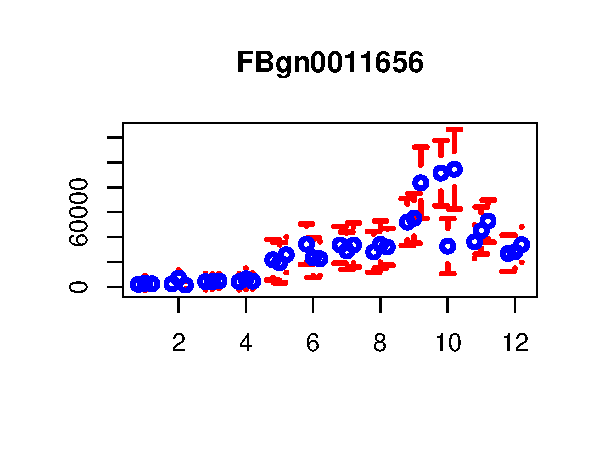
\includegraphics[width=.33\textwidth,trim=9mm 9mm 9mm 9mm]{../../../gpsim/tex/diagrams/dros_expression_series_1}
    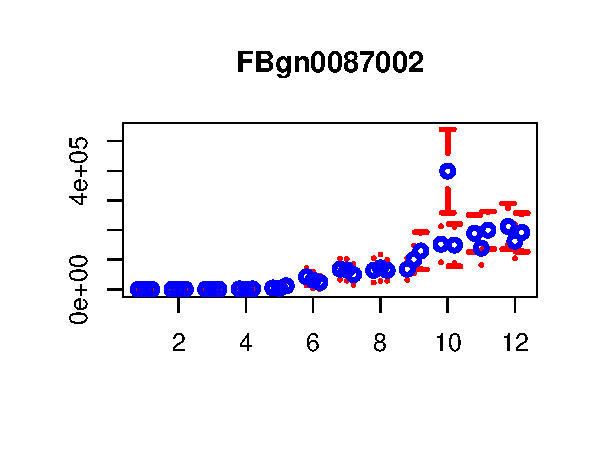
\includegraphics[width=.33\textwidth,trim=9mm 9mm 9mm 9mm]{../../../gpsim/tex/diagrams/dros_expression_series_5}
    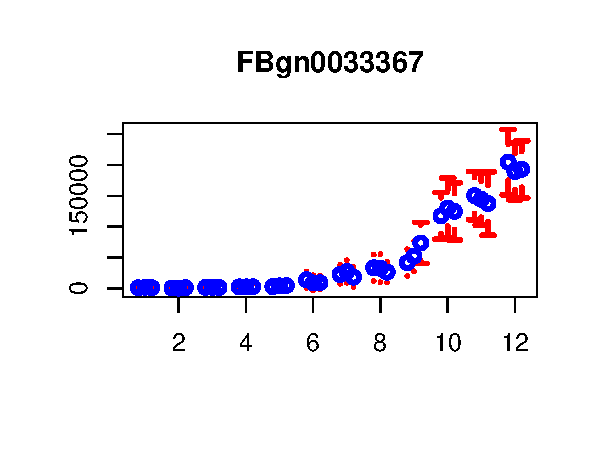
\includegraphics[width=.33\textwidth,trim=9mm 9mm 9mm 9mm]{../../../gpsim/tex/diagrams/dros_expression_series_3}\\
    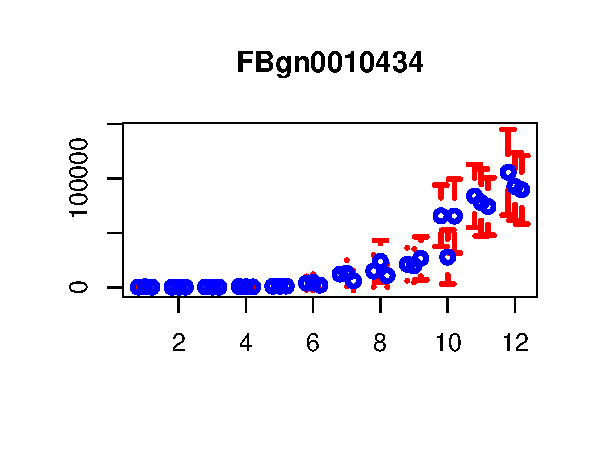
\includegraphics[width=.33\textwidth,trim=9mm 9mm 9mm 9mm]{../../../gpsim/tex/diagrams/dros_expression_series_4}
    %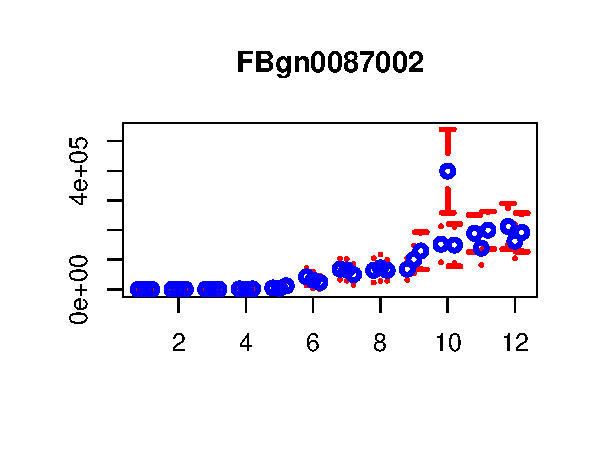
\includegraphics[width=.33\textwidth,trim=9mm 9mm 9mm 9mm]{../../../gpsim/tex/diagrams/dros_expression_series_5}
    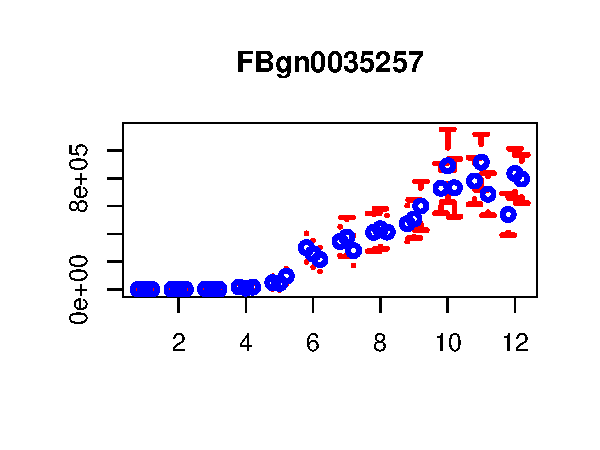
\includegraphics[width=.33\textwidth,trim=9mm 9mm 9mm 9mm]{../../../gpsim/tex/diagrams/dros_expression_series_6}
    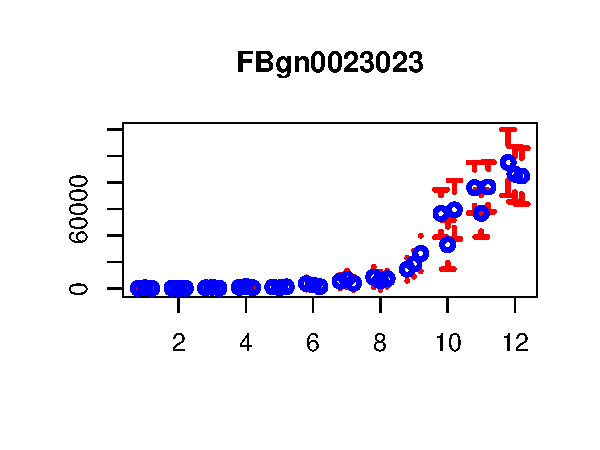
\includegraphics[width=.33\textwidth,trim=9mm 9mm 9mm 9mm]{../../../gpsim/tex/diagrams/dros_expression_series_7}\\
    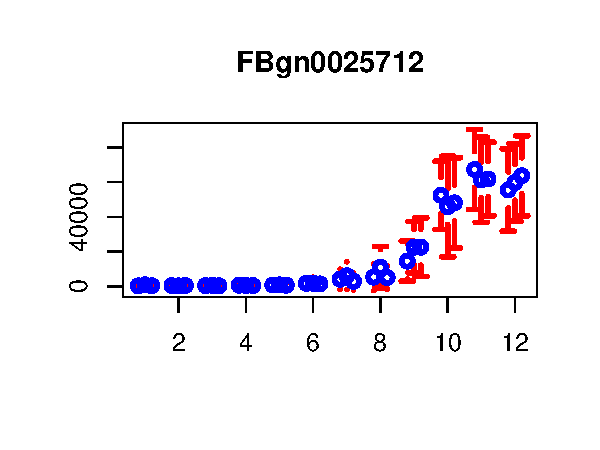
\includegraphics[width=.33\textwidth,trim=9mm 9mm 9mm 9mm]{../../../gpsim/tex/diagrams/dros_expression_series_8}
    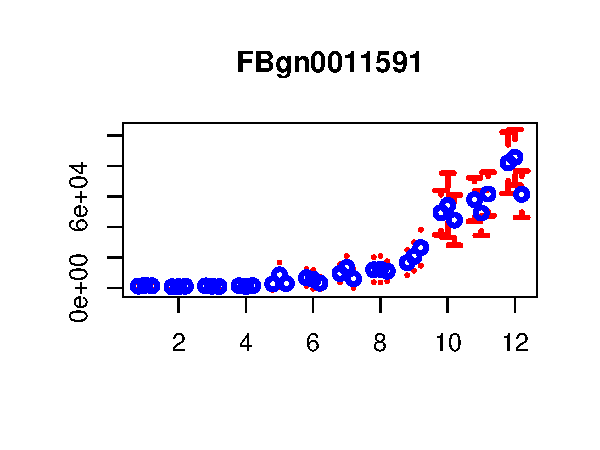
\includegraphics[width=.33\textwidth,trim=9mm 9mm 9mm 9mm]{../../../gpsim/tex/diagrams/dros_expression_series_10}
    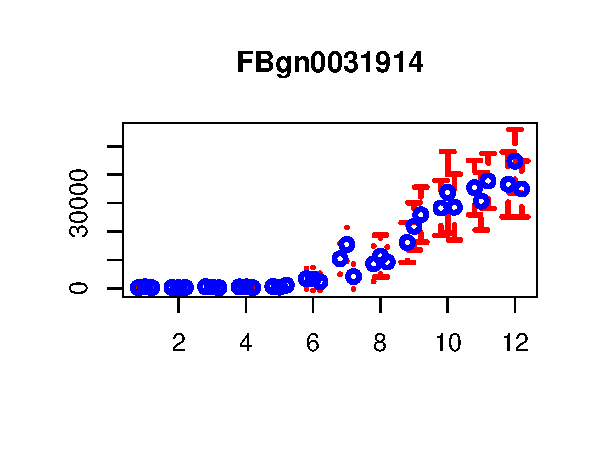
\includegraphics[width=.33\textwidth,trim=9mm 9mm 9mm 9mm]{../../../gpsim/tex/diagrams/dros_expression_series_11}
  \end{center}
}

\subsection{Models: theory}

% \frame{
%   \frametitle{Outline}

%   \tableofcontents[currentsubsection,hideothersubsections]{}
% }

\frame{
  \frametitle{Example model: Linear ODE model of transcription}

  \begin{itemize}
  \item Linear Activation Model (\citealp{Barenco:ranked06}, Genome
    Biology) \[
    \frac{\dif \mrnaConcentration_{j}\left(t\right)}{\dif t}=\basalRate_{j}+\sensitivity_{j}\tfConcentration\left(t\right)-\decayRate_{j}\mrnaConcentration_{j}\left(t\right)\]
 
  \item $\mrnaConcentration_{j}(t)$ -- concentration of gene $j$'s mRNA 
  \item $f(t)$ -- concentration of active transcription factor 
  \item Model parameters: baseline $\basalRate_{j}$, sensitivity $\sensitivity_{j}$ and
    decay $\decayRate_{j}$ 
  \item Placing a Gaussian process (GP) prior on $\tfConcentration(t)$ leads to
    a joint GP over all concentration profiles (\citealp{Gao:latent08},
    Bioinformatics)
  \end{itemize}
}

\frame{
  \frametitle{How to connect the model to data?}

  \begin{enumerate}
  \item Assume {\color{red}independent profiles} for each complete
    (biological) repeat
    \begin{itemize}
    \item Loses statistical power for extra independence assumptions
    \item Is it meaningful to order the repeats?
    \end{itemize}
  \item Assume one {\color{red}shared underlying profile} with independent
    observations
    \begin{itemize}
    \item Potentially sensitive to outliers
    \end{itemize}
  \end{enumerate}
}

\frame{
  \frametitle{Exchangeability analysis}

  Assume $\mrnaConcentration_j^k(t_i)$ observation of $k$th repeat of $j$th gene at $i$th time

  \begin{tabular}{lcc}
    & $\mrnaConcentration_:^k(t_i) \leftrightarrow \mrnaConcentration_:^{k'}(t_i)$ & $\mrnaConcentration_j^k(t_i) \leftrightarrow \mrnaConcentration_j^{k'}(t_i)$ \\
    & ``swap arrays'' & ``swap single gene'' \\
    \hline
    ``Reality'' & {\color{green}Yes} & {\color{green}No} \\
    1. Independent profiles & {\color{red}No} & {\color{green}No} \\
    2. Shared profile & {\color{green}Yes} & {\color{red}Yes} \\
  \end{tabular}
}

\frame{
  \frametitle{Solution: hierarchical GP model}

  \begin{itemize}
  \item Assume the underlying $f(t)$ is composed of a shared and an
    experiment-specific part $f_{ik}(t)$
\[
    \frac{\dif \mrnaConcentration_{j}\left(t\right)}{\dif t}=\basalRate_{j}+\sensitivity_{j}[f_{\text{shared}}\left(t\right) + f_{ik}\left(t\right)]-\decayRate_{j}\mrnaConcentration_{j}\left(t\right)
    \]
  \item Covariance is of the same form as usual
  \item Introduces additional covariance terms for measurements from
    the same experiment
  \item Alternative parametrisations of variance of $f_{ik}(t)$
    \begin{itemize}
    \item Shared across all experiments
    \item Sampled independently for each experiment
    \end{itemize}
  \end{itemize}
}

\frame{
  \frametitle{Exchangeability analysis revisited}

  Assume $\mrnaConcentration_j^k(t_i)$ observation of $k$th repeat of $j$th gene at $i$th time

  \begin{tabular}{lcc}
    & $\mrnaConcentration_:^k(t_i) \leftrightarrow \mrnaConcentration_:^{k'}(t_i)$ & $\mrnaConcentration_j^k(t_i) \leftrightarrow \mrnaConcentration_j^{k'}(t_i)$ \\
    & ``swap arrays'' & ``swap single gene'' \\
    \hline
    ``Reality'' & {\color{green}Yes} & {\color{green}No} \\
    1. Independent profiles & {\color{red}No} & {\color{green}No} \\
    2. Shared profile & {\color{green}Yes} & {\color{red}Yes} \\
    3. Hierarchical model & {\color{green}Yes} & {\color{green}No} \\
  \end{tabular}
%   \begin{tabular}{lccc}
%     & Indep.\ profiles & Shared profile & Hierarchical \\
%     $\mrnaConcentration_:^k(t_i) \leftrightarrow \mrnaConcentration_:^{k'}(t_i)$ & {\color{red}No} & {\color{green}Yes} & {\color{green}Yes} \\
%     $\mrnaConcentration_j^k(t_i) \leftrightarrow \mrnaConcentration_j^{k'}(t_i)$ & {\color{green}No} & {\color{red}Yes} & {\color{green}No} \\
%   \end{tabular}
}

\subsection{Models: practice}

% \frame{
%   \frametitle{Outline}

%   \tableofcontents[currentsection,hideothersubsections]{}
% }

\frame{
  \frametitle{ODE model of translation and transcription}

  \begin{itemize}
  \item Assume TF is transcriptionally regulated with related mRNA
    $y(t)$
  \item This yields a system of ODEs \citep{Gao:latent08}
    \begin{align*}
      \frac{\dif f\left(t\right)}{\dif t} & =\sigma y\left(t\right)-\delta f\left(t\right)\\
      \frac{\dif x_{j}\left(t\right)}{\dif t} & =\basalRate_{j}+\sensitivity_{j}f\left(t\right)-\decayRate_{j}x_{j}\left(t\right)
    \end{align*}
  \item The corresponding GP model can be derived analogously to the
    previous case
  \end{itemize}
}

\frame{
  \frametitle{Independent profiles}

  \begin{center}
    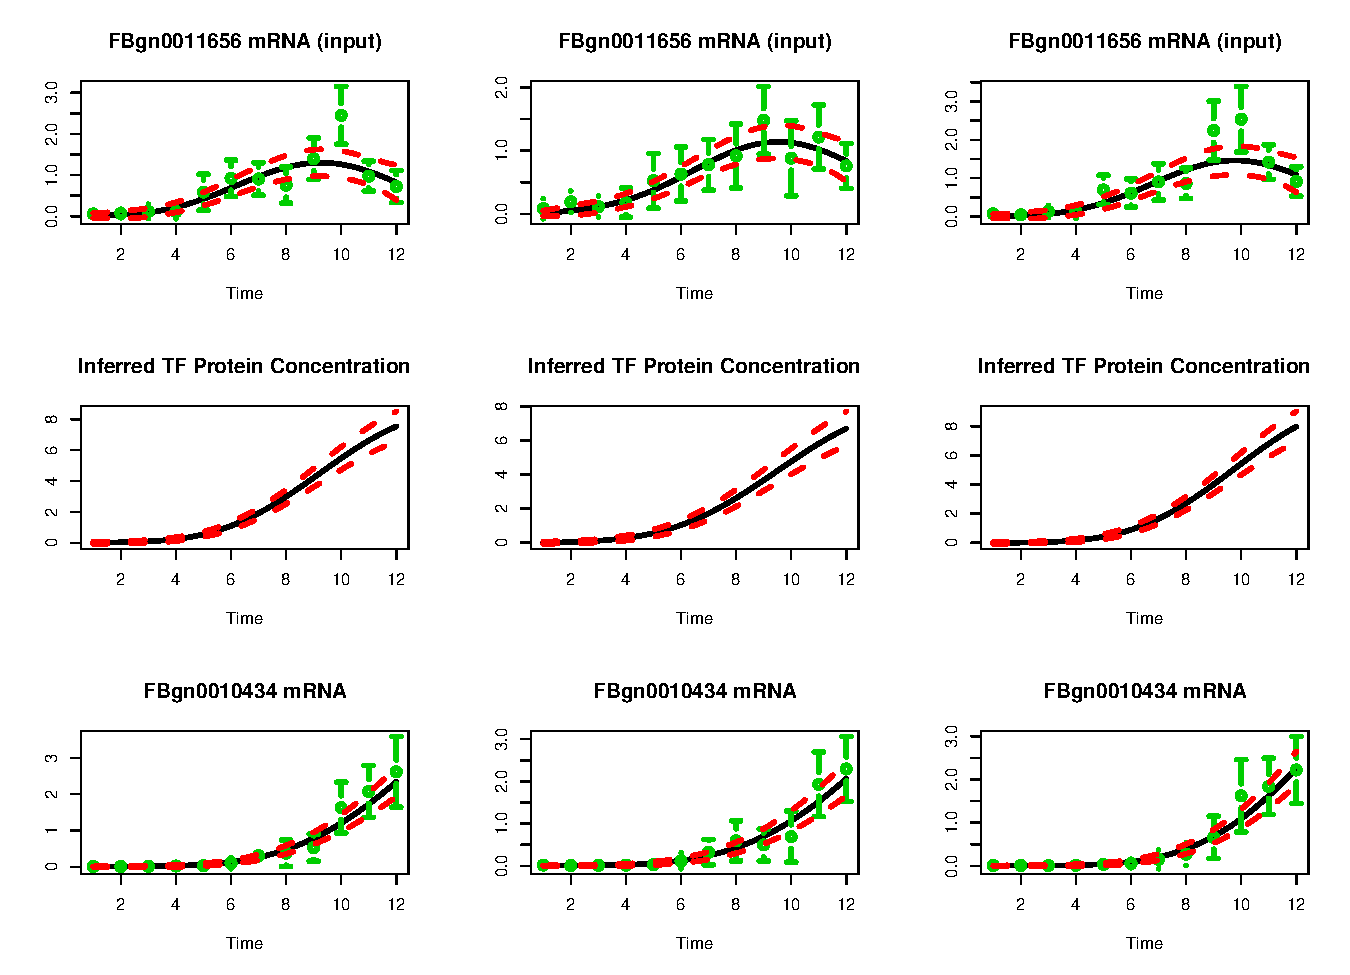
\includegraphics[scale=0.45]{../../../gpsim/tex/diagrams/old_sample_model}
  \end{center}
}

\frame{
  \frametitle{Hierarchical model}

  \begin{center}
    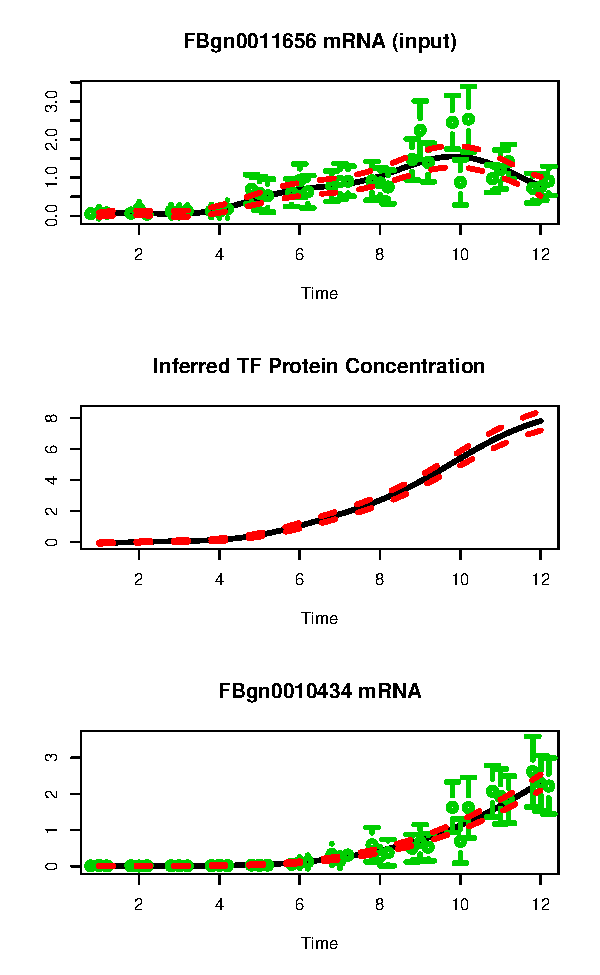
\includegraphics[scale=0.5]{../../../gpsim/tex/diagrams/hier_sample_model}
  \end{center}
}

%%% Local Variables: 
%%% mode: latex
%%% TeX-master: t
%%% End: 
